
\section{课本例题重现}

\subsection{例题1}

\begin{enumerate}
	
	\item[\textbf{L1-1}]	
	已知一质点的运动学方程为$r(t) = 2ti + (7 - 4t^2)j \quad(SI\text{单位})$,求该质点的轨迹方程.
	
	\item[\textbf{L1-2}]
	如图L1-2所示,一人通过一根不可伸缩的绳水平向右拉小车前进,绳跨过一个小定滑轮,小车位于人拉绳的一端上方高为 $h$ 的平台上,人的速率 $v_0$ 不变,求人离滑轮的水平距离为 $s$ 时,小车的速度大小和加速度大小.
	
	\begin{figure}[H]
		\centering
		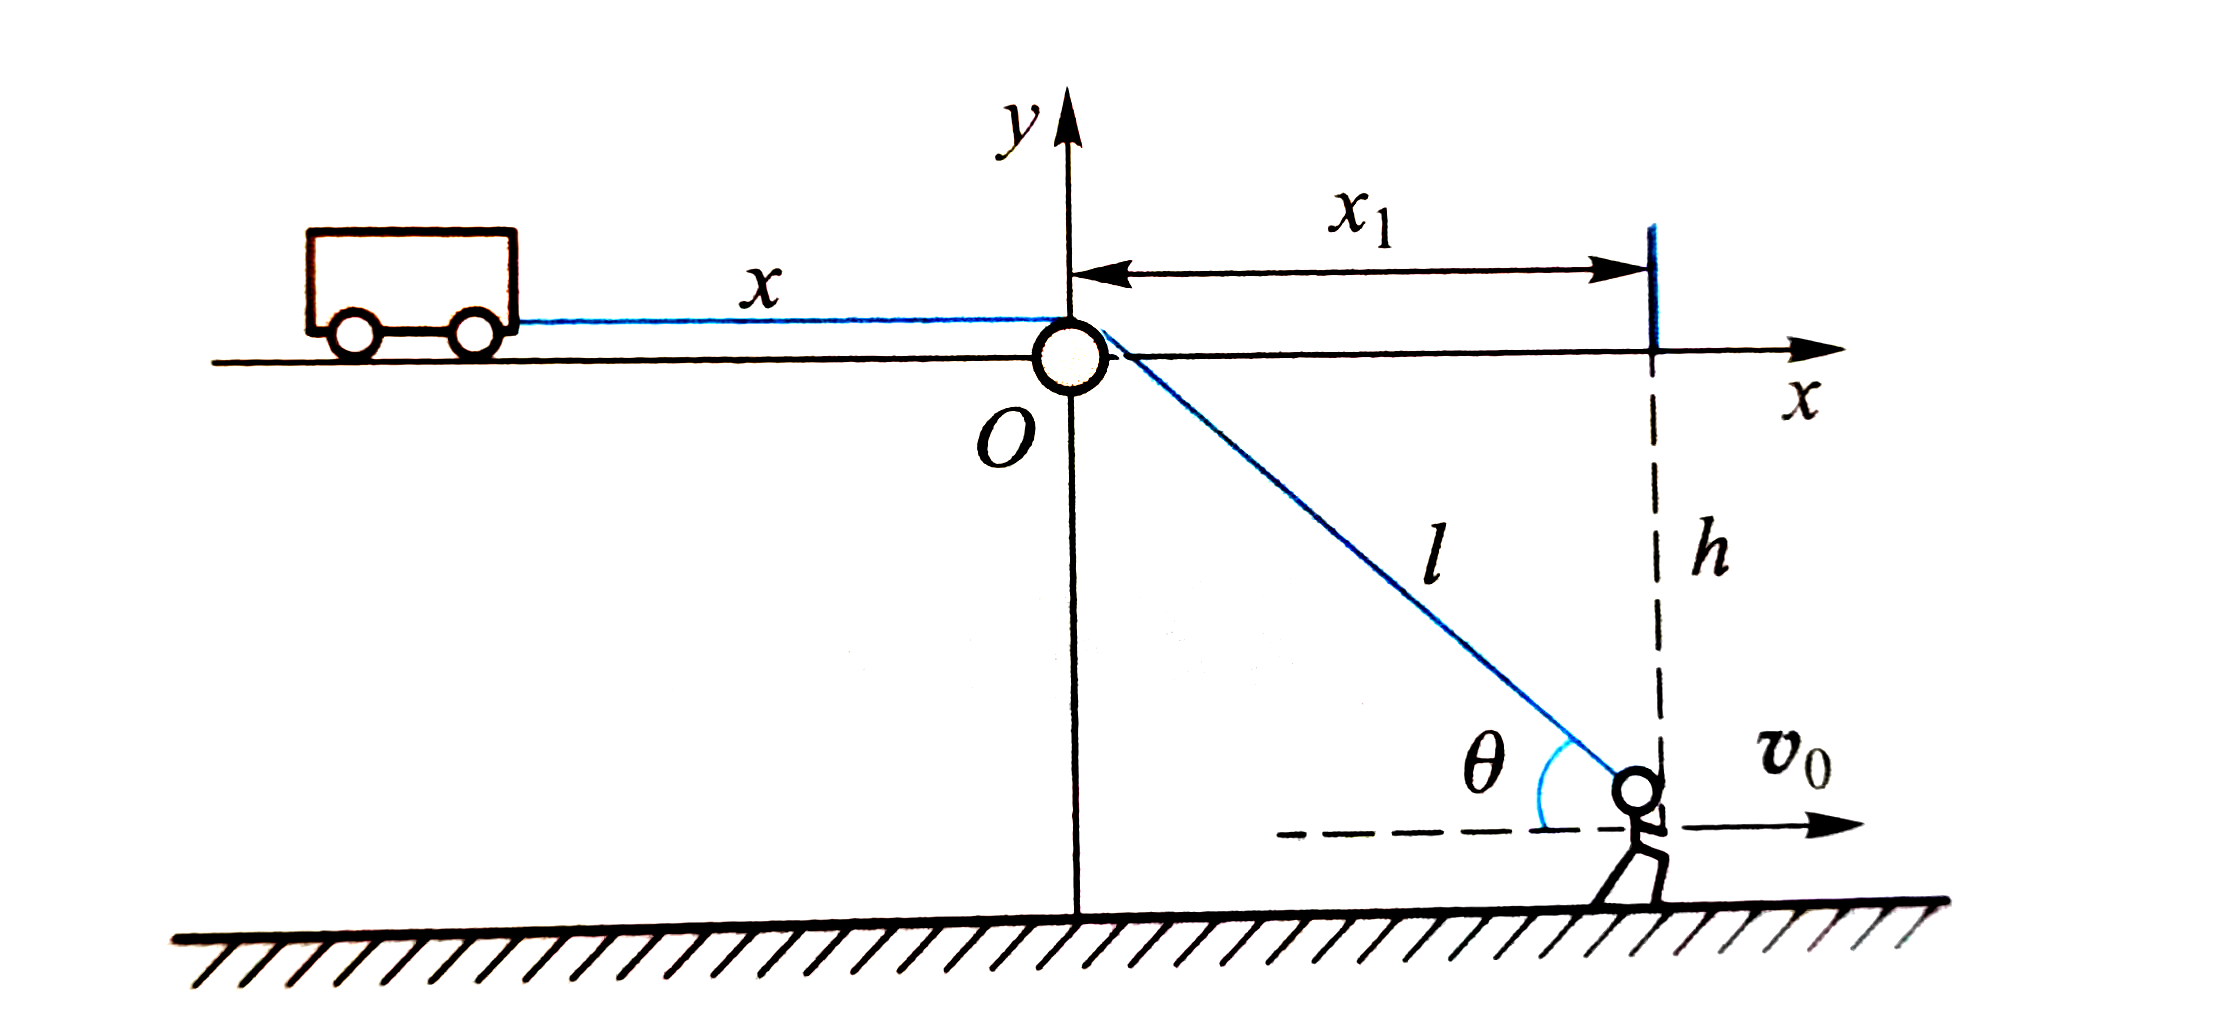
\includegraphics[width=0.3\linewidth]{figures/L1-2}
		\caption{例题L1-2图}
		\label{fig:l1-2}
	\end{figure}
	
	
	\item[\textbf{L1-3}]
	以速度 $v_0$ 平抛一小球,不计空气阻力,如图 L1-3 所示. 以平抛时为计时起点,求 $t$ 时刻小球的切向加速度分量 $a_t$ 和法向加速度分量 $a_n$,以及轨迹的曲率半径 $\rho$.
	
	\begin{figure}[H]
		\centering
		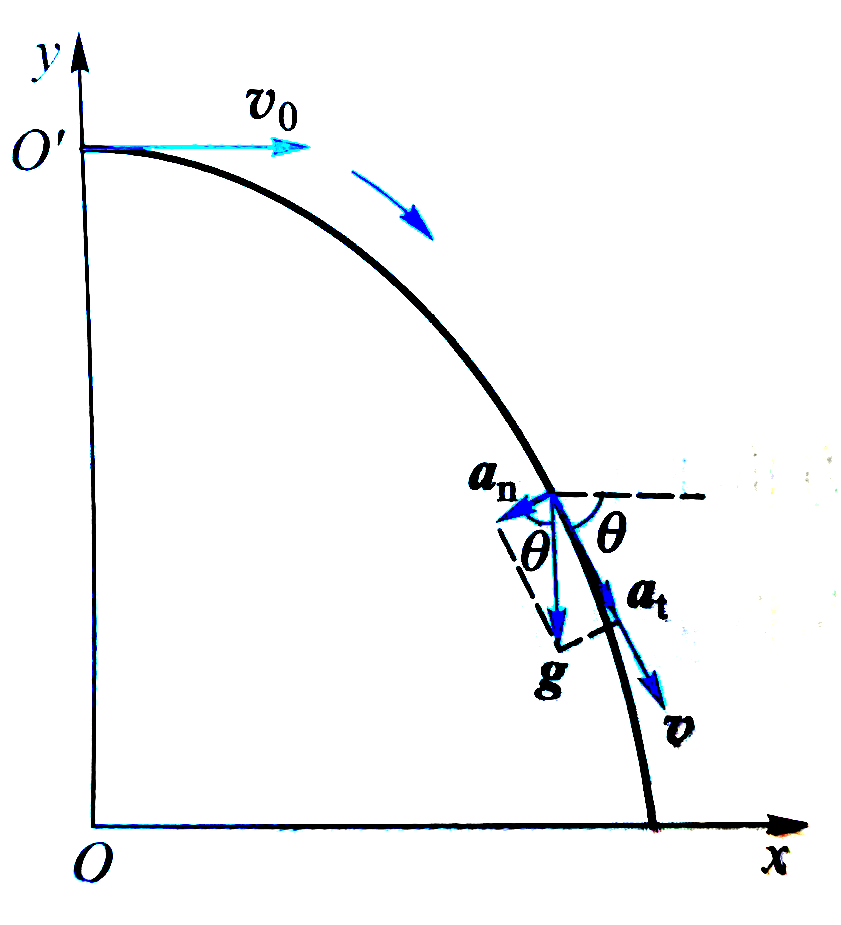
\includegraphics[width=0.3\linewidth]{figures/L1-3}
		\caption{例题L1-3图}
		\label{fig:l1-3}
	\end{figure}
	
	
	
	\item[\textbf{L1-4}]
	一飞轮以初始转速 $n = 1\,500 \mathrm{\ r \cdot min^{-1}}$ 转动,受制动后均匀地减速,经 $t = 50 \mathrm{\ s}$ 后静止. 
	
	\begin{enumerate}
		
		\item 求角加速度 $\alpha$；
		\item 从开始制动到静止,飞轮转过的转数 $N$；
		\item 制动开始后 $20 \mathrm{\ s}$ 时飞轮的角速度
		\item 设飞轮半径为 $R = 0.60 \mathrm{\ m}$,求 $t = 20 \mathrm{\ s}$ 时刻飞轮边缘上任一点的速率和加速度大小.
		
	\end{enumerate}
	
	
	\item[\textbf{L1-5}]
	已知质点的运动学方程为 $\boldsymbol{r} = 2t\boldsymbol{i} + (8 - 6t^2)\boldsymbol{j}$ (SI 单位),求:
	
	\begin{enumerate}
		\item 质点运动轨迹方程；
		\item 从 $t_1 = 1\mathrm{\ s}$ 到 $t_2 = 2\mathrm{\ s}$ 这段时间内质点的位移、平均速度；
		\item 在任意时刻的速度、加速度；
		\item 在任意时刻的切向加速度、法向加速度.
		
	\end{enumerate}
	
	
	\item [\textbf{L1-6}]
	一质点沿一半径为 $R = 1 \mathrm{\ m}$ 的圆周运动,其角量运动学方程为 $\theta = 2 + t + 3t^3$ (SI 单位). 求:
	
	\begin{enumerate}
		\item $t = 1 \mathrm{\ s}$ 时,质点的角位置、角速度、角加速度；
		\item $t = 1 \mathrm{\ s}$ 时,质点的速率、切向加速度、法向加速度和加速度大小.
	\end{enumerate}
	
	
	\item [\textbf{L1-7}]
	已知质点的加速度为 $\boldsymbol{a} = 2\boldsymbol{i} + 6t^2\boldsymbol{j}$ (SI 单位),初始时刻 ($t=0$) 质点位于坐标原点处,初速度为 $\boldsymbol{v}_0 = 2\boldsymbol{i} \mathrm{\ m \cdot s^{-1}}$. 求:
	
	\begin{enumerate}
		
		\item 质点在任意时刻的速度；
		\item 运动学方程 $\boldsymbol{r}(t)$ 和轨迹方程.
		
	\end{enumerate}
	
	
\end{enumerate}

\subsection{例题2}

\begin{enumerate}
	\item
\end{enumerate}


\subsection{例题7}

\begin{enumerate}
	
	\item 
	
\end{enumerate}



\subsection{例题8}

\begin{enumerate}
	
	\item 
\end{enumerate}









% 需要宏包：booktabs, tabularx, array
\section{其他题目}

\begin{enumerate}

\item[\textbf{1-7}] 质点做直线运动,\textbf{r}表示位置矢量,\textbf{v}表示速度,\textbf{a}表示加速度,\textbf{s}表示 路程,$a_t$表示切向加速度,下列表达式中,(\quad)

(1). $\dfrac{dv}{dt} = a$,
(2). $\dfrac{{dr}}{dt} = {v}$,
(3). $\dfrac{ds}{dt} = v$,
(4). $\left| \dfrac{d\mathbf{v}}{dt} \right| = a$.

\begin{choices}
	\item 只有\(1\)、\(4\)是对的.
	\item 只有\(2\)、\(4\)是对的.
	\item 只有\(2\)是对的.
	\item 只有\(3\)是对的.
\end{choices}






\end{enumerate}